\section{Eksperyment 4: Efektywność wyszukiwania}

Eksperyment 1 porównywał metody po wykorzystaniu całego budżetu 300 modeli. Celem
eksperymentu 4 jest sprawdzenie, jak szybko każda metoda dochodzi do dobrego wyniku:
ilu ocenionych modeli i ile czasu treningu potrzebuje, żeby osiągnąć określoną jakość,
oraz czy ACO mogłoby osiągnąć wynik Random Search przy mniejszym budżecie.

\subsection{Konfiguracja}

Eksperyment nie wymagał nowych konfiguracji. Analiza obejmuje przebiegi eksperymentu 1
(trzy warianty feromonów i Random Search, trzy zbiory, 10 ziaren, parametry domyślne).
Ponieważ potrzebne są pełne zapisy przebiegów, czyli kolejność ocen, najlepszy dotychczasowy
wynik i czas treningu każdej sieci, wszystkie 120 przebiegów powtórzono lokalnie na
procesorze, dla tej samej wersji kodu i tego samego pliku konfiguracyjnego. Każdy przebieg
liczył się w osobnym procesie na jednym wątku (12 procesów równolegle na jednym komputerze),
więc czasy treningu są porównywalne między strategiami. Tak małe sieci uczą się na jednym
wątku procesora szybciej niż na karcie Tesla T4: łączny czas treningu przebiegu Random Search
na zbiorze Letter Recognition wyniósł ok.~17 minut wobec ok.~36 minut na Kaggle
(tab.~\ref{tab:e1-summary}).

Obliczenia na GPU i CPU nie są bitowo zgodne, dlatego średnie dokładności różnią się od
wartości z tabeli~\ref{tab:e1-summary}: walidacyjne o nie więcej niż 0,0023, a testowe o nie
więcej niż 0,006. Powtórzenie potwierdziło
wnioski eksperymentu 1: żadna z dziewięciu różnic dokładności testowej między wariantem ACO
a Random Search nie jest istotna po korekcie Holma.

Efektywność opisano trzema miarami:
\begin{itemize}
    \item $b(k)$ -- najlepsza dokładność walidacyjna po $k$ ocenionych modelach (krzywa
    z rys.~\ref{fig:e1-conv}). Dla $k \in \{50, 100, 200, 300\}$ każdy wariant ACO porównano
    z Random Search dwustronnym testem U Manna-Whitneya na wartościach z 10 ziaren, z korektą
    Holma na dziewięć porównań dla każdego $k$.
    \item Liczba modeli i czas do osiągnięcia poziomu Random Search, czyli średniej wartości
    $b(300)$ Random Search na danym zbiorze. Dla każdego przebiegu wyznaczono pierwszy model,
    po którym $b(k)$ osiąga ten poziom, oraz łączny czas treningu do tego momentu, wyrażony
    jako procent średniego czasu treningu całego przebiegu Random Search.
    \item Koszt pojedynczego modelu: średnia liczba warstw ukrytych i średni czas treningu
    jednej sieci.
\end{itemize}

\subsection{Wyniki}

Rysunek~\ref{fig:e4-adv} przedstawia różnicę między średnią krzywą zbieżności każdego
wariantu ACO a krzywą Random Search, a tabela~\ref{tab:e4-budget} wartości $b(k)$ dla
wybranych budżetów. Przewaga ACO pojawia się w pierwszych kilkudziesięciu modelach. Na
zbiorze Letter Recognition jest największa już po ok.~30--50 modelach, na zbiorze Wine
Quality rośnie do ok.~200 modeli, a pod koniec wyszukiwania na obu zbiorach maleje, bo
Random Search powoli nadrabia dystans. Na zbiorze Wine Quality przewaga jest największa
przy budżecie 200 modeli (0,62--0,74 punktu procentowego)
i dla wszystkich trzech wariantów istotna przy $k = 100$ i $k = 200$, a przy $k = 300$
już tylko dla wariantu \texttt{independent}. Na zbiorze Letter Recognition warianty
\texttt{param\_dependent} i \texttt{independent} mają przewagę ok.~0,5 punktu procentowego,
istotną od $k = 100$ do końca wyszukiwania, a \texttt{config\_dependent} mniejszą
i nieistotną. Na zbiorze Adult różnica nie przekracza 0,07 punktu procentowego i przy
żadnym budżecie nie jest istotna. Przy budżecie 50 modeli żadna różnica nie jest istotna,
przy 100 i 200 modelach istotnych jest pięć z dziewięciu, a przy 300 modelach trzy. Porównanie
po pełnym budżecie zaniża więc przewagę ACO w samym wyszukiwaniu. Po 100 modelach warianty ACO
mają na zbiorze Wine Quality średnio 0,581, czyli prawie tyle, ile Random Search po 300 modelach
(0,5815), a na zbiorze Letter Recognition \texttt{param\_dependent} po 100 modelach (0,9694)
przewyższa wynik końcowy Random Search (0,9668).

\begin{figure}[H]
    \centering
    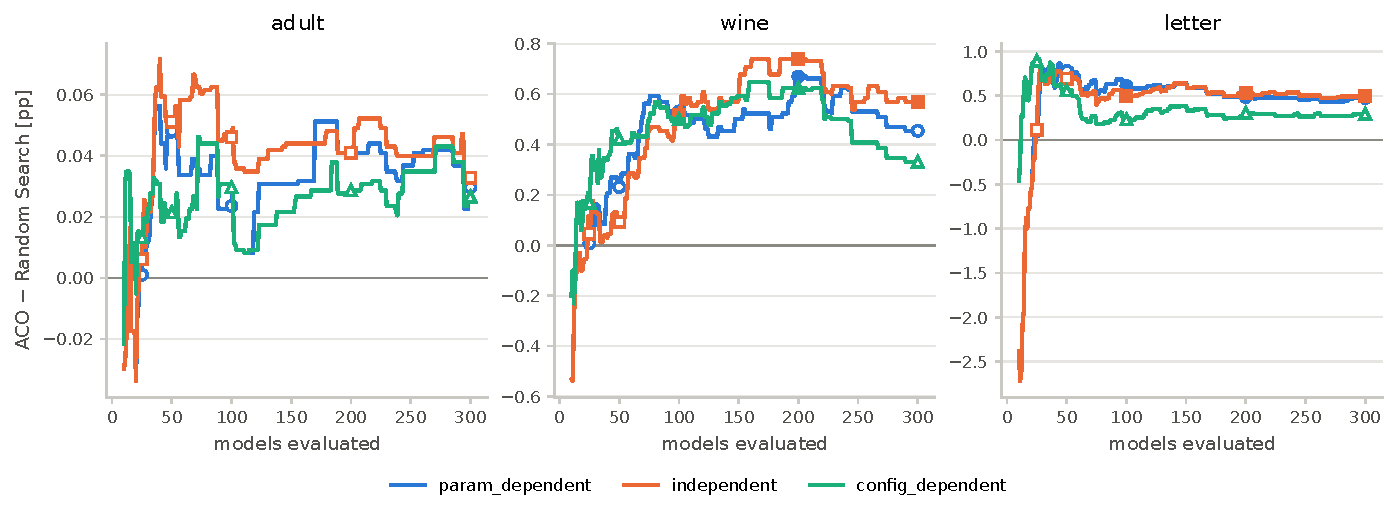
\includegraphics[width=\textwidth]{img/e4/advantage}
    \caption{Różnica między najlepszą dokładnością walidacyjną wariantu ACO a Random Search
    w funkcji liczby ocenionych modeli, w punktach procentowych (średnie z 10 ziaren, od
    10.~modelu). Pełny znacznik: różnica istotna przy tym budżecie po korekcie Holma, pusty:
    nieistotna.}
    \label{fig:e4-adv}
\end{figure}

\begin{table}[H]
    \centering
    \small
    \begin{tabular}{llrrrr}
\toprule
zbiór & strategia & $k = 50$ & $k = 100$ & $k = 200$ & $k = 300$ \\
\midrule
adult & random & 0.8619 & 0.8623 & 0.8626 & 0.8630 \\
adult & param\_dependent & +0.05 & +0.02 & +0.04 & +0.03 \\
adult & independent & +0.05 & +0.05 & +0.04 & +0.03 \\
adult & config\_dependent & +0.02 & +0.03 & +0.03 & +0.03 \\
\midrule
wine & random & 0.5749 & 0.5761 & 0.5784 & 0.5815 \\
wine & param\_dependent & +0.23 & \textbf{+0.53} & \textbf{+0.67} & +0.45 \\
wine & independent & +0.09 & \textbf{+0.52} & \textbf{+0.74} & \textbf{+0.57} \\
wine & config\_dependent & +0.42 & \textbf{+0.50} & \textbf{+0.62} & +0.33 \\
\midrule
letter & random & 0.9569 & 0.9633 & 0.9658 & 0.9668 \\
letter & param\_dependent & +0.78 & \textbf{+0.61} & \textbf{+0.48} & \textbf{+0.47} \\
letter & independent & +0.69 & \textbf{+0.50} & \textbf{+0.53} & \textbf{+0.49} \\
letter & config\_dependent & +0.56 & +0.24 & +0.31 & +0.29 \\
\bottomrule
\end{tabular}
    \caption{Najlepsza dokładność walidacyjna po $k$ ocenionych modelach (średnia z 10 ziaren).
    Dla Random Search podano wartość, dla wariantów ACO różnicę względem Random Search
    w punktach procentowych. Pogrubienie: różnica istotna według testu U Manna-Whitneya po
    korekcie Holma (9 porównań dla każdego $k$, $\alpha = 0{,}05$).}
    \label{tab:e4-budget}
\end{table}

Rysunek~\ref{fig:e4-target} pokazuje, po ilu modelach poszczególne przebiegi osiągają
poziom Random Search. Na zbiorach Wine Quality i Letter Recognition warianty
\texttt{param\_dependent} i \texttt{independent} dochodzą do niego w 9--10 przebiegach na 10,
w medianie po 70--99 modelach. Wariant \texttt{config\_dependent} jest wolniejszy (mediana
114--115 modeli, 8 przebiegów na 10). Sam Random Search osiąga własny średni wynik końcowy
tylko w 4--5 przebiegach na 10, zwykle po 146--256 modelach. Na zbiorze Adult różnice są
mniej wyraźne: warianty ACO osiągają ten poziom w 5--9 przebiegach na 10, w medianie po
102--123 modelach, a Random Search w 4 przebiegach.

\begin{figure}[H]
    \centering
    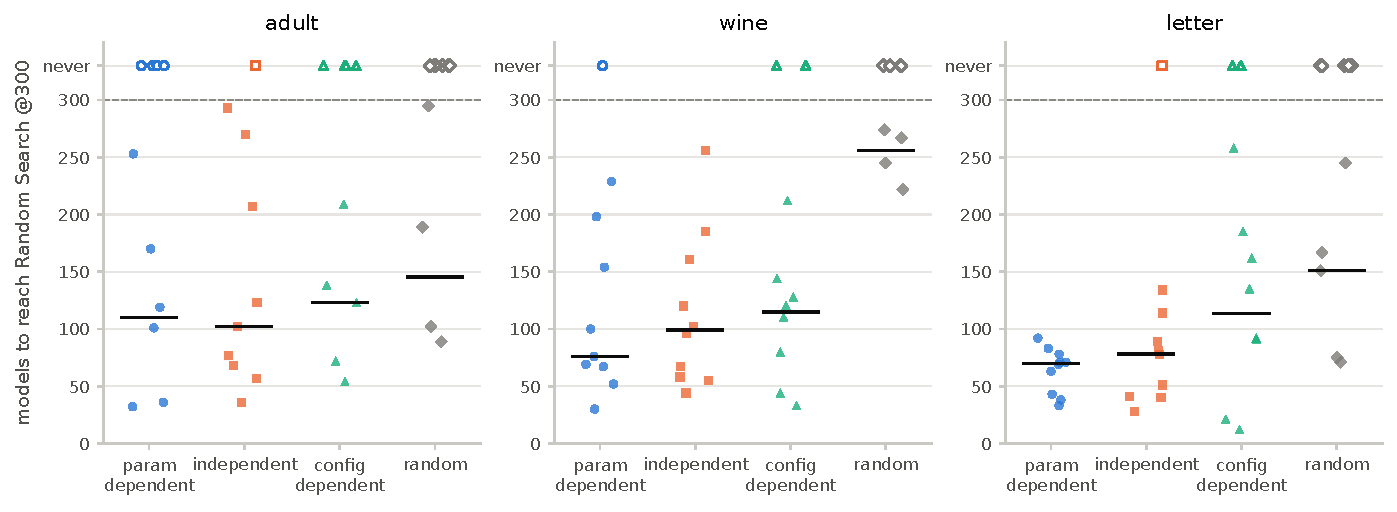
\includegraphics[width=\textwidth]{img/e4/to_target}
    \caption{Liczba ocenionych modeli, po której przebieg osiąga średni wynik końcowy Random
    Search na danym zbiorze. Punkt to jedno ziarno, kreska to mediana przebiegów, które ten
    poziom osiągnęły. Puste znaczniki (\emph{never}) oznaczają przebiegi, które go nie
    osiągnęły w ramach budżetu 300 modeli.}
    \label{fig:e4-target}
\end{figure}

Wyższa skuteczność ma swój koszt (tab.~\ref{tab:e4-cost}). Na zbiorach Wine Quality i Letter
Recognition kolonia buduje średnio głębsze sieci niż Random Search (2,2--2,8 warstwy wobec
1,9), a na zbiorze Adult sieci podobnej głębokości. Na procesorze czas treningu rośnie
z rozmiarem sieci, więc przebieg ACO trwa dłużej o 7--12\% na zbiorze Adult, o 15--25\% na
Wine Quality i o 29--62\% na Letter Recognition. Na kartach T4 ta sama różnica wynosiła tylko
5--15\% (tab.~\ref{tab:e1-summary}), bo czas treningu tak małych sieci na GPU zależy głównie
od stałego narzutu na każdą paczkę danych, a mniej od ich rozmiaru. Mimo droższych modeli
warianty \texttt{param\_dependent} i \texttt{independent} dochodzą do poziomu Random Search
w 27--39\% czasu, jaki Random Search zużywa na cały przebieg, na zbiorach Wine Quality
i Letter Recognition. Na zbiorze Adult jest to 35--51\%, czyli tyle, ile zużywają nieliczne
przebiegi Random Search, które ten poziom osiągnęły.

\begin{table}[H]
    \centering
    \small
    \begin{tabular}{llrrrrrr}
\toprule
zbiór & strategia & warstwy & s/model & czas vs RS & przebiegi & modele & czas \\
\midrule
adult & param\_dependent & 1.96 & 4.80 & +12\% & 6/10 & 110 & 42\% \\
adult & independent & 1.88 & 4.59 & +7\% & 9/10 & 102 & 35\% \\
adult & config\_dependent & 1.99 & 4.66 & +9\% & 5/10 & 123 & 51\% \\
adult & random & 1.91 & 4.29 & -- & 4/10 & 146 & 49\% \\
\midrule
wine & param\_dependent & 2.48 & 1.04 & +21\% & 9/10 & 76 & 30\% \\
wine & independent & 2.84 & 1.07 & +25\% & 10/10 & 99 & 39\% \\
wine & config\_dependent & 2.31 & 0.98 & +15\% & 8/10 & 115 & 42\% \\
wine & random & 1.91 & 0.86 & -- & 4/10 & 256 & 85\% \\
\midrule
letter & param\_dependent & 2.34 & 4.93 & +49\% & 10/10 & 70 & 27\% \\
letter & independent & 2.51 & 5.39 & +62\% & 9/10 & 78 & 29\% \\
letter & config\_dependent & 2.24 & 4.27 & +29\% & 8/10 & 114 & 46\% \\
letter & random & 1.91 & 3.32 & -- & 5/10 & 151 & 48\% \\
\bottomrule
\end{tabular}
    \caption{Koszt i szybkość wyszukiwania (10 ziaren, CPU, jeden wątek na przebieg). Kolumny:
    średnia liczba warstw ukrytych ocenianych sieci, średni czas treningu jednej sieci,
    łączny czas treningu przebiegu względem Random Search, liczba przebiegów, które osiągnęły
    średni wynik końcowy Random Search, oraz mediana liczby modeli i czasu (jako procent
    średniego czasu przebiegu Random Search) potrzebnych do jego osiągnięcia, liczona wśród
    tych przebiegów.}
    \label{tab:e4-cost}
\end{table}

Na efektywność wpływają też powtórzenia. Ponieważ każda sieć jest uczona od zera, ponowna
ocena tej samej architektury zużywa budżet bez poszerzania przeszukanej przestrzeni. Na
zbiorze Adult warianty ACO oceniają średnio 178--183 różne architektury na 300, mniej niż
Random Search (208). Na zbiorach Wine Quality i Letter Recognition jest odwrotnie (203--249),
bo kolonia przechodzi do głębszych sieci, a Random Search połowę ocen poświęca sieciom
jednowarstwowym, których jest tylko 80.

\subsection{Wnioski}

Pod względem samego wyszukiwania ACO jest wyraźnie efektywniejsze od Random Search na
zbiorach Wine Quality i Letter Recognition. Warianty \texttt{param\_dependent}
i \texttt{independent} osiągają wynik końcowy Random Search w medianie po 70--99 modelach
i w 27--39\% jego czasu, mimo że trenują droższe sieci. Średnio po 100 modelach mają tyle,
ile Random Search po 300, choć rozrzut między ziarnami jest duży (rys.~\ref{fig:e4-target}).
Przewaga jest istotna przy budżetach 100--200 modeli, a przy pełnym budżecie częściowo maleje,
bo Random Search powoli nadrabia dystans. Wariant \texttt{config\_dependent} jest
wolniejszy, co jest zgodne z obserwacjami z eksperymentu 2: najbardziej szczegółowa
reprezentacja feromonów potrzebuje najwięcej ocen, żeby się czegoś nauczyć. Na zbiorze Adult,
gdzie wiele architektur osiąga niemal tę samą dokładność, żadna metoda nie zyskuje wiele,
a ACO dodatkowo częściej ocenia te same sieci.

Koszt pojedynczego modelu zależy od sprzętu: głębsze sieci wybierane przez kolonię wydłużają
przebieg na procesorze o 7--62\%, a na GPU tylko o 5--15\%. W obu przypadkach ACO dochodzi
do dobrego wyniku w krótszym czasie niż Random Search.

Efektywność mierzona była na zbiorze walidacyjnym, czyli na kryterium, które optymalizują
mrówki. Eksperyment 1 pokazał, że przewaga na walidacji nie przenosi się na zbiór testowy.
ACO znajduje więc równie dobre sieci szybciej, a nie sieci lepsze.
